\scanpage{24}
\mspage{\handwritten{15}}
$p$-linéaire\handwritten{s} opérant sur les $H^i(X,\underline{O}_X)$. Quitte à remplacer $k$ par une extension finie, on peut supposer que toutes les valeurs propres desdits frobenius sont égales à 0 ou 1. Soit $c$ la somme alternée \deleted{\unsure{des valeurs} valeurs des du nombre} des rangs semi-simples des $H^i(X,\underline{O}_X)$ pour $0\handwritten{\leq}i\handwritten{\leq}n-1$. Alors pour toute extension finie $k'$ de $k$, la somme alternée des traces de $\operatorname{frob}_{k'}$ opérant sur les $H^i(X_{k'},\underline{O}_{X_{k'}})$ est \deleted{alors}\deleted{\handwritten{\unsure{encore}}} égale à $c$. En vertu de Lefschetz-Verdier Deligne, et des isomorphismes (**), on conclut que pour tout point $s\handwritten{\in}U(k')$, on a
\[
\operatorname{card}Y_{\unsure{s|t}}(k')\equiv c+(-1)^{n-1}\operatorname{Tr}f_s\,,
\tag*{\deleted{\unsure{***|xxx}}}
\]
où $f_s\handwritten{\in}G_o$ est \deleted{l'image de l'élément de Frobenius de} le frobenius relatif à $k'$ opérant sur $E_o(Y_s)$. Ceci posé, 7.1 est une conséquence des deux lemmes suivants;

\margin{\figure{\begin{tikzpicture}[x=1cm,y=1cm]\node at (0,0.3) {\handwritten{!}};\draw (0.45,-0.8)--(0.52,1.5);\end{tikzpicture}}}
\uline{Lemme} 7.5. Pour tout $s\handwritten{\in}U$, il existe un élément $f\handwritten{\in}G_o$ \inserted{\handwritten{et $V'_o\subset V_o$ \unsure{stable} par $f$}} tel que le polynôme caractéristique de $f$ opérant sur \figure{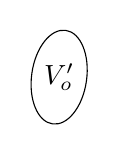
\begin{tikzpicture}\node at (0,0) {$V_o^{\handwritten{\prime}}$};\draw[rotate=-8] (0,0) ellipse (0.35cm and 0.6cm);\end{tikzpicture}} soit égal à celui de $f_s$, et en particulier tel que $f\handwritten{|_{V'_o}}$ et $f_s$ aient même trace.

\uline{Lemme} 7.6. Pour tout entier $N\handwritten{\geq}0$, il existe un entier $d^{\handwritten{\prime}}_o$ \inserted{\handwritten{$>0$}} tel que pour tout entier $d\handwritten{\geq}d'_o$, il existe une extension finie $k'$ de $k$ et un point $s\handwritten{\in}U_d(k')$ tel que $\operatorname{card}(Y_s)=N$. (Marche dès que $X$ est un sous-schéma fermé de $P^r_k$ de dimension $n\handwritten{\geq}1$.)

\uline{Démonstration de} 7.6. \inserted{\handwritten{On peut supposer $X$ réduit.}} Soit $r$ la \inserted{somme des} degrés des composantes irréductibles réduites de $X$ qui sont de\deleted{d} dimension $n$, et soit $d_1$ un entier tel que
\[
N\handwritten{\geq}rd_1^n\,.
\]
Quitte à passer à une extension finie de $k$, on peut supposer \deleted{que chaque composante irréductible $X_i$ de $X$ \inserted{est géom. irréductible et} contient un point rationnel sur $k$ qui\unsure{\,$x_i$} n'appartient à aucune et que} les composantes irréductibles $X_i$ de $X$ géométriquement irréductibles, que tout $X_i$ contient un $x_i\handwritten{\in}X_i(k)$, et qu'il existe $n$ formes $\handwritten{\phi}_o,\ldots,\handwritten{\phi}_{n-1}$ de degré $d_1$ sur $P^r_k$,
% archive sheet number: 23
